\problemname{Mirror Madness}

Yesterday, a new attraction was opened at the local funfair: a hall of mirrors.
This is a labyrinth in which all the walls are covered with mirrors so that
visitors lose their sense of direction in a sea of reflections. The layout of
the labyrinth can be described by a polygon with all sides parallel to either
the x-axis or y-axis.
\medskip

On the opening day, many visitors got so lost that the ride operators had to
intervene and help them find their way out. To better understand where visitors
get lost the most, the operators decided to install a monitoring system. This
system involves an invisible laser beam running through the hall of mirrors at
foot level, so that the movement of the visitors can be tracked by observing
when and where the laser beam gets interrupted.
\medskip

The laser beam starts at some boundary point of the polygon at an angle of $45$
degrees to the wall. Whenever it hits a mirror, it bounces off in a $90$ degree
angle. To get their monitoring system to work, the operators are planning to
install sensors at each of the first $m$ bouncing points of the laser beam.
Find the locations where the sensors need to be installed.
\bigskip

\begin{figure}[!h]
  \centering
  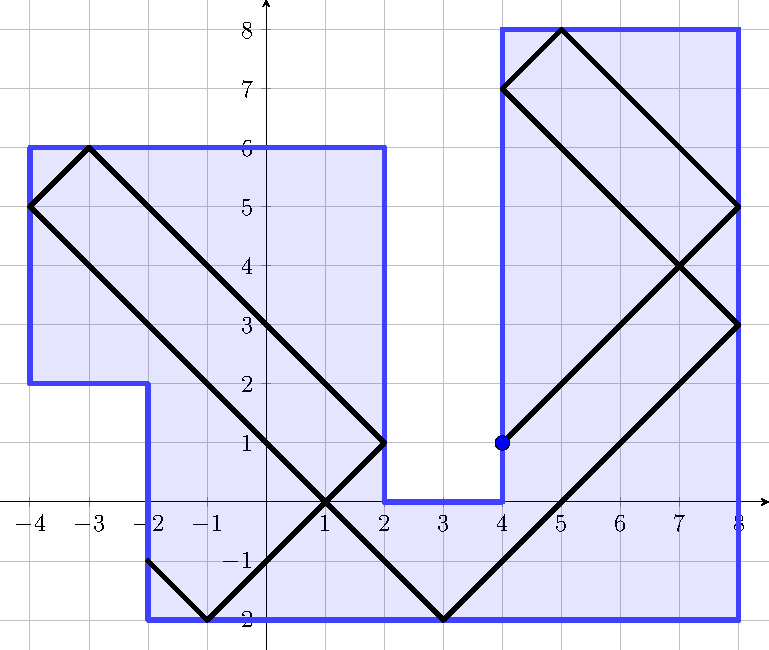
\includegraphics[width=0.6\textwidth]{sample2}
  \caption{Illustration of the second sample case.}
\end{figure}
\bigskip

\begin{Input}
	The input consists of:
  \begin{itemize}
    \item One line with two integers $n$ and $m$ ($1 \le n,m \le 5\cdot 10^5$),
      the number of vertices of the polygon and the number of bounces.
    \item $n$ lines, each with two integers $x$ and $y$ giving the coordinates of one vertex.
    \item One line with integers $x_s$ and $y_s$, the coordinates of the starting point.
  \end{itemize}
  \newpage
  Additionally, the input satisfies the following constraints:
  \begin{itemize}
    \item The vertices of the polygon are given in counterclockwise order.
    \item The edges of the polygon do not touch or intersect each other, except
      for consecutive edges, which share their endpoints.
    \item The edges of the polygon alternate between horizontal and vertical.
    \item The perimeter (the total length of all sides) of the polygon does not
      exceed $10^6$.
    \item All coordinates in the input have absolute value at most $10^6$.
    \item All coordinates of the vertices of the polygon and exactly one
      coordinate of the starting point are even (so the laser never hits a
      vertex of the polygon).
    \item The starting point is on the boundary of the polygon.
    \item The initial direction of the laser beam is $(1,1)$, and this points
      inside the polygon.
  \end{itemize}
\end{Input}

\begin{Output}
  Output $m$ lines, each with two integers $x$ and $y$, giving the coordinates
  of the bounce locations in order.
\end{Output}
